\documentclass[11pt]{article}
\usepackage{latexsym}
\usepackage{amssymb,amsmath}
\usepackage[pdftex]{graphicx}
% \usepackage{qtree}
\usepackage{enumerate}

\topmargin = -.75in \textwidth=7in \textheight=9.3in
\oddsidemargin = -.3in \evensidemargin = -.3in

\begin{document}
\begin{center}
\large
CS181 Assignment 3
\end{center}
Joy Ming and Alisa Nguyen (15 March 2013)\\

\section{Problem 1}
\begin{enumerate}[a.]
\item The probability that all of the $M$ dimensions of $x - y$ are between $-\epsilon \text{ and } \epsilon$ is \fbox{$ \rho = (2\epsilon)^M$}.
\\ For each dimension $i$ of $\chi$, the probability that $|x_i - y_i| \leq \epsilon$ is equivalent to
\begin{center}
$P(|x_i - y_i| \leq \epsilon) = $ \\
$P(- \epsilon \leq x_i - y_i \leq \epsilon) = $ \\
$P(- \epsilon - x_i \leq - y_i \leq \epsilon - x_i) = $ \\
$P(\epsilon + x_i \geq y_i \geq x_i - \epsilon) = $ \\
$P(x_i - \epsilon \leq y_i \leq \epsilon + x_i)$
\end{center}
This distribution function is equivalent to $\int_{\epsilon + x_i}^{x_i - \epsilon} f(x)dx$, where $f(x)$ is the PDF of $y_i$, which we know to have a uniform distribution, so $f(x) = \frac{1}{b - a} = 1$. Thus, we get:
\begin{center}
$\int_{\epsilon + x_i}^{x_i - \epsilon} 1 dx = $ \\
$\epsilon + x_i - (x_i - \epsilon) = 2\epsilon$
\end{center}
Because we want to know the probability that all of the $M$ dimensions of $x - y$ are between $-\epsilon$ and $\epsilon$, we simply take $\Pi_{i = 1}^{M} P(|x_i - y_i| \leq \epsilon) = (2\epsilon)^M$.
\item The probability of $max_m |x_m - y_m| \leq \epsilon$ is at most $\rho$ because as shown in (a), $\rho$ does not depend on $x_i$ and thus holds for all $x_i$. In addition, logically, if $x$ is the center point, the average distance from it to any other point $y$ is at most $\frac{1}{2}$ for any one dimension. As $x$ moves farther and farther away from the center, the average distance increases so that it becomes at most 1 in any one dimension. So, if $x$ is not in the center $max_m|x_m - y_m|$ grows and is less likely to be less than $\epsilon$, decreasing that probability so that it is less than $\rho$.
\item We will show that $||x - y|| \geq max_m|x_m - y_m|$.
\begin{center}
$||x - y|| = \sqrt{\Sigma_{m = 1}^{M} (x_m - y_m)^2} $ \\
$\sqrt{\Sigma_{m = 1}^{M} (x_m - y_m)^2} \geq max_m|x_m - y_m|$ \\
$\Sigma_{m = 1}^{M} (x_m - y_m)^2 \geq (max_m|x_m - y_m|)^2$
\end{center}
This is true because the left side of the inequality includes the right side in its sum. $|| x - y ||$ is the total Euclidean distance between two points whereas $max_m|x_m - y_m|$ is only the distance between one dimension of two points. The left side must be larger.
\newline \newline
If $x$ is any point in $\chi$, and $y$ is a point in $\chi$ drawn randomly from a uniform distribution on $\chi$, then the probabilty that $||x - y|| \leq \epsilon$ is also at most $p$ because $||x - y||$ is greater than or equal to $max_m|x_m - y_m|$, making it less likely to be less than $\epsilon$ and thus giving it a probability lower than $\rho$ of being less than $\epsilon$.
\item Lowerbound on number $N$ of points needed to guarantee that the nearest neighbor of point $x$
 will be within a radius $\epsilon$ of it is \fbox{$log\delta / log(1 - (2\epsilon)^M)$}.
\newline
For the nearest neighbor not to be within a radius $\epsilon$, none of the neighbors can be within a radius $\epsilon$. The probability that any one neighbor is not within a radius $\epsilon$ of $x$ is $1 - (2\epsilon)^M$, so the probability that all the nighbors are not within a radius $\epsilon$ of $x$ is equivalent to $(1 - (2\epsilon)^M)^N$, where $N$ is the number of neighbors. So, the probability that at least one neighbor is within a radius $\epsilon$ is 1 - that quantity. Since we want to guarantee with probability at least $1 - \delta$ that the nearest neighbor will be within a radius $\epsilon$ of it, we can solve for a lower bound for N by setting the two equations equal to each other.
\begin{center}
$1 - \delta = 1 - (1 - (2\epsilon)^M)^N$ \\
$1 - 1 + (1 - (2\epsilon)^M)^N = \delta$ \\
$(1 - (2\epsilon)^M)^N = \delta $ \\
$Nlog(1 - (2\epsilon)^M) = log\delta$ \\
\fbox{$N = log\delta/log(1 - (2\epsilon)^M)$}
\end{center}
\item We can conclude that the effectiveness of the hierarchical agglomerative clustering algorithm in high dimensional spaces is ineffective as the dimension $M$ grows because $N$ would also grow too large and HAC would require too many $N$ points to actually be effective. As $M$ increases, the denominator of the lower bound for $N$ decreases, thus leading to an increase in $N$ overall. In addition, as covered in class, when the size of the dataset gets larger, the probability that two points from different clusters are closer to each other in terms of distance than two points from separate clusters converges to 1/2.
\end{enumerate}

\section{Problem 2}
\begin{enumerate}[a.]
\item Given a prior distribution $Pr(\theta)$ and likelihood $Pr(D|\theta)$, the predictive distribution $Pr(x|D)$ for a new datum,
\begin{enumerate}
\item ML: $Pr(x|D)=Dist(\underset{\theta}{\arg\max}(\ln(Pr(D|\theta))))$, \\where $Dist()$ is a distribution applied to the $\theta$ we obtain with the given formula.
\item MAP: $Pr(x|D)=Dist(\underset{\theta}{\arg\max}(\ln(P(D|\theta)P(\theta))))$, \\where $Dist()$ is a distribution applied to the $\theta$ we obtain with the given formula.
\item FB: $Pr(x|D)=\int p(x|\theta) P(\theta|D)d\theta$
\end{enumerate}
\item MAP can be considered "more Bayesian" than ML because it takes into account the probability distribution of $\theta$, the prior, instead of assuming same weight or uniformity.
\item One advantage the MAP method enjoys over the ML method is that it accounts for the more likely distribution, as opposed to simply assuming uniformity, as with ML. FB, on the other hand, maintains a probability distribution over the set of all possible  parameter values. However, because the normalizing factor contains an integration over all parameter values, it can be difficult to compute. This means that it also unnecessarily takes into account the less likely, meaning that FB is less practical than MAP to calculate. Therefore, MAP sits in the "sweet spot" of taking more into account in terms of distribution than ML but less excessively than FB.
\item Soccer team example based on different Beta distributions as priors for the probability of a win, the different possible distributions are:
\begin{itemize}
\item Beta(1,1)\\
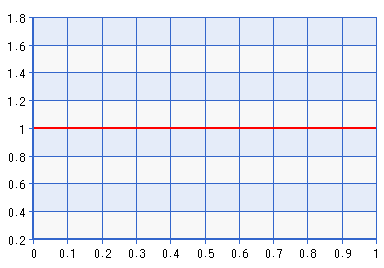
\includegraphics[width=50mm]{beta11.png}\\
The Beta(1,1) distribution is equated with the Uniform(0,1) distribution, which is a number uniformly chosen between 0 and 1. Beta(1,1) is a uniform prior on $\theta$ which says there was just one positive and one negative example, essentially makes the probability of winning and losing equally likely. Often used as a "non-informative prior", this assumes uniformity and is not very descriptive in depicting the distribution of wins and losses otherwise.
\item Beta(3,3)\\
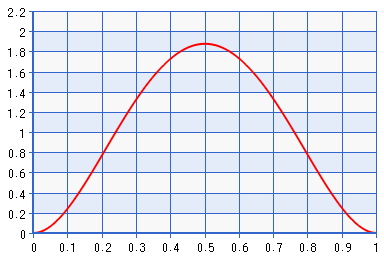
\includegraphics[width=50mm]{beta33.png}\\
Based on the equation for the mode of a variate with a beta distribution, $x = \frac{\alpha - 1}{\alpha + \beta - 2}=\frac{3-1}{3+3-2}=\frac{2}{4}$. This means that this distribution says that it is as likely to win as it is to lose as the distribution is symmetrical. However, this is more descriptive than simply a Beta(1,1) distribution, as seen in the plot because it looks more at the distribution over the entire space, with a lower variance as it makes values in the middle more likely.
\item Beta(2,5)\\
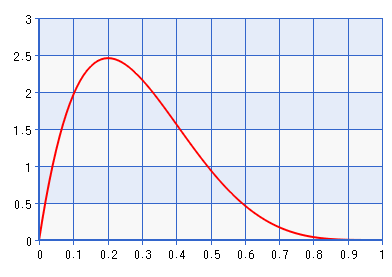
\includegraphics[width=50mm]{beta25.png}\\
In this case, the plot seems to be skewed toward the left, which the equation for the mode of a variate with a beta distribution show $x = \frac{\alpha - 1}{\alpha + \beta - 2}=\frac{2-1}{2+5-2}=\frac{1}{5}$ that this is true. This is more descriptive than Beta(1,1) in describing a distribution that is not necessarily uniform and it is also more more descriptive than Beta(3,3) in describing a distribution that is not necessarily as symmetrical.
\end{itemize}
\item The Beta distribution is the conjugate prior of the Bernoulli, so it is useful when used together with MAP estimation with Bernoulli variables since the posterior and prior will then have the same form. We can use this conjugate relationship to more easily use MAP estimation. 
\item Looking at the Harvard football team in the 2011-2012 season,
	\begin{itemize}
	\item Using the ML approach, we basically take the naive probability looking at the number of wins over the total number of games, so the probability they would win is $\frac{9}{10}$. So, we predict that they will \fbox{win} next after the first three games of the 2012-2013 season.
	\item Using the MAP approach, we take into account the prior distribution, assuming a Beta distribution of Beta($\alpha,\beta$), \[\theta_{MAP} = \frac{n_w+\alpha-1}{n+\alpha+\beta-2}\]. Guessing the same prior we guess in class of Beta(5,3), which can be interpreted as though more winds than losses have been observed in the past, the equation becomes
	\[\theta_{MAP} = \frac{n_w+\alpha-1}{n+\alpha+\beta-2}=\frac{5+9-1}{10+5+3-2}=\frac{13}{16}\]. Beta(5,3) is good because it accounts for complications about uniformity and symmetry. Because the probability is higher than 1/2,we predict that they will \fbox{win} the next game.
	\item Using the FB approach, we integrate over the entire distribution, 
	\end{itemize}
\end{enumerate}

\section{Problem 3}
\begin{enumerate}[a.]
\item The $K$-means clustering objective is to minimize the sum of squared distances between prototype and data. The update steps can be derived by performing gradient descent on it by taking the partial derivative over all means and responsibilities. This means we can move along the negative gradient of the loss function, as shown in the lecture slides to converge to a local minimum. Each iteration of the K-means algorithm updates the prototypes to decrease the error, following gradient descent until the prototypes converge to a local minimum and the loop ends. Because each iteration does decrease the error, K-means is guaranteed to converge in the direction that decreases the error the most, or in the direction of steepest descent. 
\item The principal components analysis (PCA), which looks to compress features using a linear reduction into lower dimension space, has an interpretation that looks to minimize the difference between data points through minimum square loss. One way they are related is that principal components are the continuous solutions to the discrete cluster membership indicators for $K$-means clustering. As PCA can be represented by a covariance matrix, $K$-means can be represneted by a spectral expansion of the data covariance matrix truncated at $k$-1 terms. The relaxed solution of $k$-means clustering is given by the PCA principal components, where the PCA subspace spanned by the principal directions is identical to the cluster centriod subspace.\\
Some example situations and hypothetical data sets include:
	\begin{itemize}
	\item PCA appropriate
	\item $K$-means appropriate
	\end{itemize}
\end{enumerate}

\section{Problem 4}
\begin{enumerate}[a.]
\item $K$-means clustering algorithm
\begin{enumerate}
\item Plot of mean squared error versus $K$\\
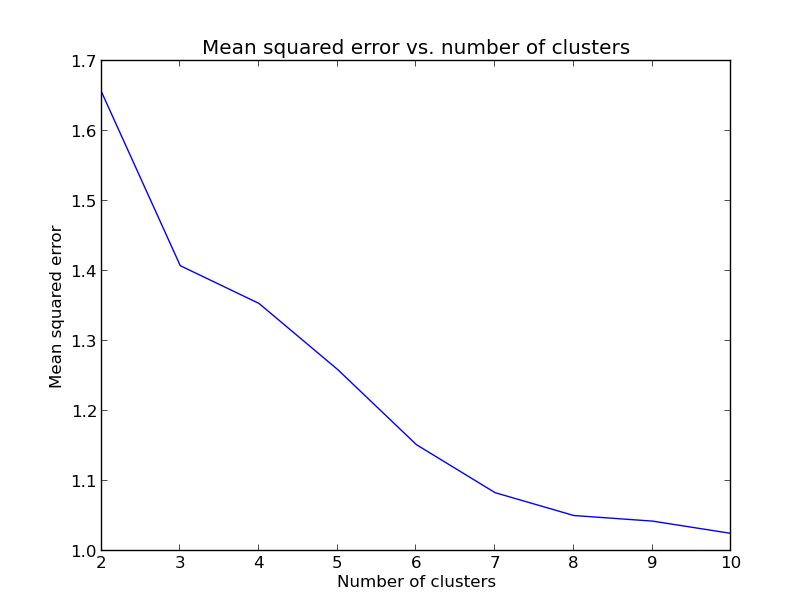
\includegraphics[width=120mm]{graphkmeans.png}
\item If we were to chose the best $K$ for this data based onthe plot generated in part (i) we would chose the value of $K$ that minimizes the mean squared error, which in this case is 10. It is important to minimize mean squared error because it is a measure of the difference between estimated values and true values, following in line with objectives mentioned in problem 3. 
\end{enumerate}
\item HAC algorithm
\begin{enumerate}
\item Comparing clusters formed using $min$ distance metric against clusters formed using $max$ distance metric
\begin{enumerate}
\item Table showing number of instances in each cluster\\
\begin{tabular}{|c|c|c|c|c|}
\hline
Metric & C1 & C2 & C3 & C4\\ \hline
$min$ & 1 & 1 & 73 & 25\\ \hline
$max$ & 7 & 21 & 46 & 26\\
\hline
\end{tabular}
\item Scatterplot of the instances in 3-dimensions
	\begin{itemize}
	\item Based on $min$:\\
	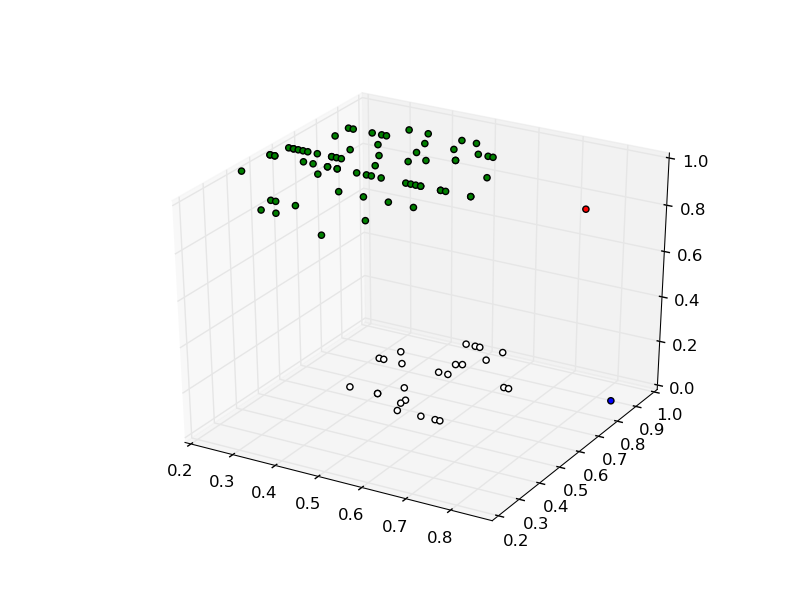
\includegraphics[width=120mm]{graphhac.png}
	\item Based on $max$:\\
	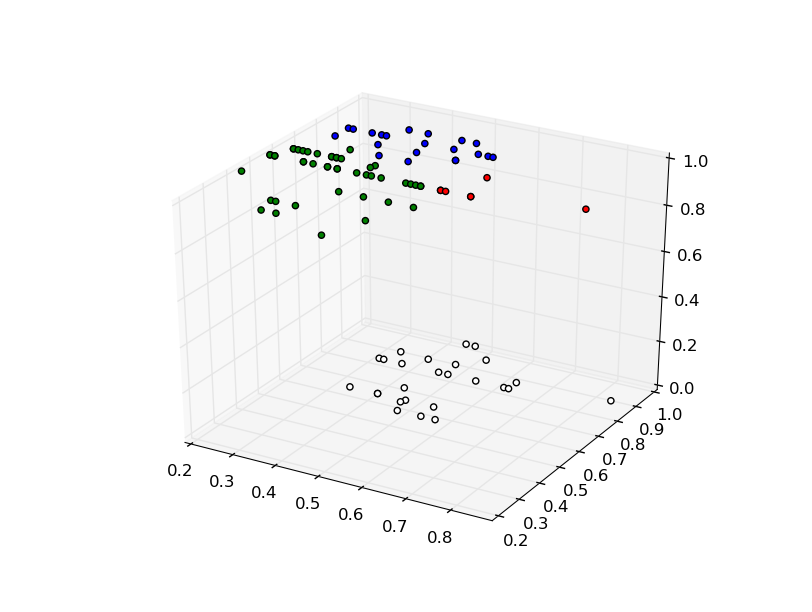
\includegraphics[width=120mm]{graphhacmax.png}
	\end{itemize}
\end{enumerate}
The $min$ distance metric considers the distance between the two closest points in two separate clusters, but the $max$ distance metric considers the distance between the two farthest points in the clusters. This results in the $min$ measure creating more distinct and consolidated clusters than the $max$ metric, which makes sense because by minimizing the smallest distance this brings the points closer to each other.
% It seems that the $min$ distance metric produced ?? clusters compared to the $max$ metric... This makes sense given the definition of the metrics because...
\item Comparing clusters formed using $mean$ distance metric against clusters formed using $centroid$ distance metric
\begin{enumerate}
\item Table showing number of instances in each cluster\\
\begin{tabular}{|c|c|c|c|c|}
\hline
Metric & C1 & C2 & C3 & C4\\ \hline
$mean$ & 1 & 1 & 46 & 152\\ \hline
$cent$ & 1 & 5 & 147 & 47\\
\hline
\end{tabular}
\item Scatterplot of the instances in 3-dimensions
\begin{itemize}
	\item Based on $mean$:\\
	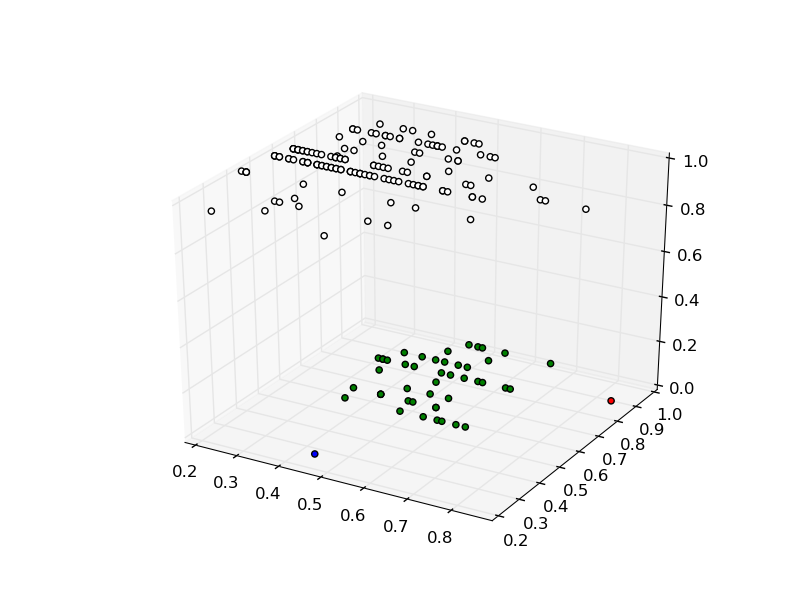
\includegraphics[width=120mm]{graphhacmean.png}
	\item Based on $cent$:\\
	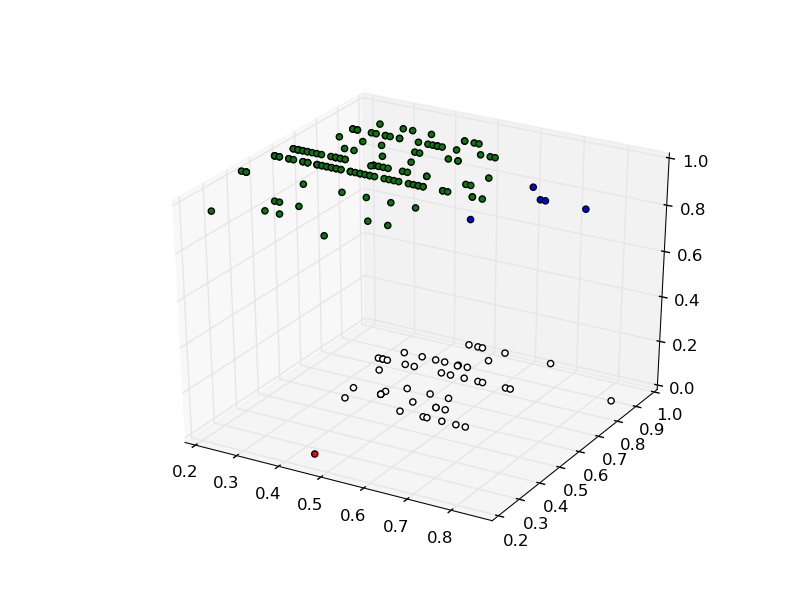
\includegraphics[width=120mm]{graphhaccent.png}
	\end{itemize}
\end{enumerate}
The $mean$ distance metric looks at the average distances between each of the points in a cluster and $cent$ looks at the distances to the center of a cluster. In the clusters based on $mean$ the clusters are more distinct in a naive belief of what the clusters would look like whereas the $cent$ is a little different and less distinct.
\end{enumerate}

\item Autoclass clustering algorithm
\begin{enumerate}
\item It takes $x$ number of iterations for the parameters to converge.
\item Plot of the log likelihood of the data versus number of iterations
\item The run-time performance of auto-class seems to be much faster than that of $K$-means. (???)
\end{enumerate}
\end{enumerate}

\end{document}